% Clean hierarchical redraw of plots/mismatch/2_1/hybrid_network_2_1.gml
% (same graph as hybrid_network_2_1.tex, but laid out top-down as a tree
%  plus one highlighted reticulation/hybridization edge, with short IDs).
% Compile with: pdflatex hybrid_network_2_1_clean.tex
\documentclass{article}
\usepackage[margin=1cm]{geometry}
\usepackage{tikz}
\usetikzlibrary{arrows.meta}

% matplotlib tab:blue / tab:orange, matching the gene_color values in the GML
\definecolor{tabblue}{rgb}{0.12156863,0.46666667,0.70588235}
\definecolor{taborange}{rgb}{1.0,0.49803922,0.05490196}

\begin{document}
\thispagestyle{empty}
\begin{center}
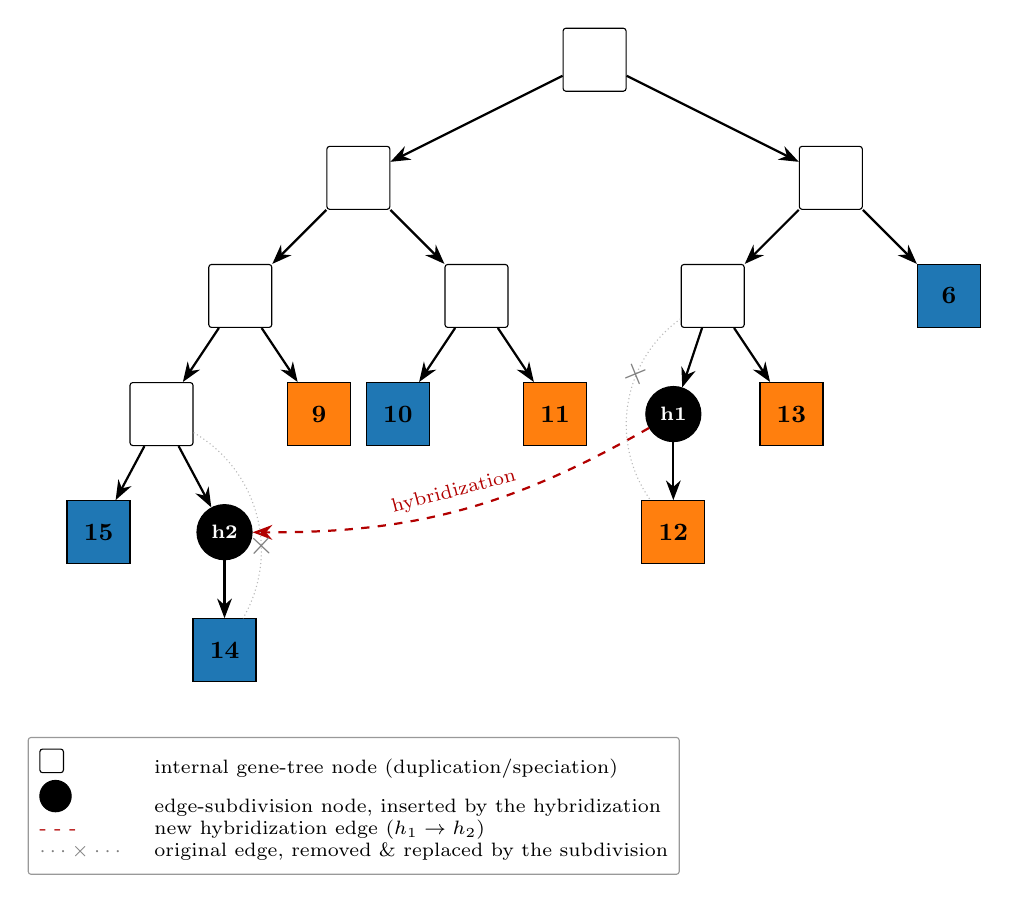
\begin{tikzpicture}[
  >={Stealth[length=2.5mm]},
  every node/.style={font=\small\bfseries},
  internal/.style={rectangle, fill=white, text=black, minimum size=8mm, draw=black, rounded corners=1pt},
  leafblue/.style={rectangle, fill=tabblue, text=black, minimum size=8mm, draw=black},
  leaforange/.style={rectangle, fill=taborange, text=black, minimum size=8mm, draw=black},
  hybrid/.style={circle, fill=black, text=white, minimum size=7mm, draw=black, font=\scriptsize\bfseries},
  treeedge/.style={->, thick},
  hybedge/.style={->, thick, dashed, red!70!black},
  removededge/.style={-, thin, gray!55, densely dotted},
]

% ---- level 0: root ----
\node[internal] (v1) at (6, 0)     {};

% ---- level 1 ----
\node[internal] (v2) at (3, -1.5)  {};
\node[internal] (v3) at (9, -1.5)  {};

% ---- level 2 ----
\node[internal]   (v4)  at (1.5, -3) {};
\node[internal]   (v5)  at (4.5, -3) {};
\node[internal]   (v6)  at (7.5, -3) {};
\node[leafblue]    (l6)  at (10.5, -3) {6};

% ---- level 3 ----
\node[internal]   (v7)  at (0.5, -4.5) {};
\node[leaforange] (l9)  at (2.5, -4.5) {9};
\node[leafblue]    (l10) at (3.5, -4.5) {10};
\node[leaforange] (l11) at (5.5, -4.5) {11};
\node[hybrid]      (h1)  at (7.0, -4.5) {h1};
\node[leaforange] (l13) at (8.5, -4.5) {13};

% ---- level 4 ----
\node[leafblue]    (l15) at (-0.3, -6) {15};
\node[hybrid]      (h2)  at (1.3, -6) {h2};
\node[leaforange] (l12) at (7.0, -6) {12};

% ---- level 5 ----
\node[leafblue]    (l14) at (1.3, -7.5) {14};

% ---- tree edges ----
\draw[treeedge] (v1) -- (v2);
\draw[treeedge] (v1) -- (v3);
\draw[treeedge] (v2) -- (v4);
\draw[treeedge] (v2) -- (v5);
\draw[treeedge] (v3) -- (v6);
\draw[treeedge] (v3) -- (l6);
\draw[treeedge] (v4) -- (v7);
\draw[treeedge] (v4) -- (l9);
\draw[treeedge] (v5) -- (l10);
\draw[treeedge] (v5) -- (l11);
\draw[treeedge] (v6) -- (h1);
\draw[treeedge] (v6) -- (l13);
\draw[treeedge] (v7) -- (l15);
\draw[treeedge] (v7) -- (h2);
\draw[treeedge] (h1) -- (l12);
\draw[treeedge] (h2) -- (l14);

% ---- the one reticulation / hybridization edge ----
\draw[hybedge] (h1) to[bend left=15] node[midway, above, sloped, font=\scriptsize, text=red!70!black] {hybridization} (h2);

% ---- original edges removed by hybridization (each was subdivided by inserting a hybrid node) ----
\draw[removededge] (v6) to[bend right=45]
  node[pos=0.35, sloped, font=\large, gray, inner sep=0pt] {$\times$} (l12);
\draw[removededge] (v7) to[bend left=45]
  node[pos=0.65, sloped, font=\large, gray, inner sep=0pt] {$\times$} (l14);

% ---- legend ----
\node[anchor=north west, font=\scriptsize, align=left, draw=black!40, fill=white, inner sep=4pt, rounded corners=1pt]
  at (-1.2, -8.6) {%
  \begin{tabular}{@{}ll@{}}
    \tikz\node[internal, minimum size=3mm]{}; & internal gene-tree node (duplication/speciation) \\
    \tikz\node[hybrid, minimum size=3mm, font=\tiny]{}; & edge-subdivision node, inserted by the hybridization \\
    \textcolor{red!70!black}{- - -} & new hybridization edge ($h_1 \to h_2$) \\
    \textcolor{gray}{$\cdots\times\cdots$} & original edge, removed \& replaced by the subdivision \\
  \end{tabular}%
};

\end{tikzpicture}
\end{center}
\end{document}
